\chapter{ペトリネット変換に基づく二段階最適化}
\label{main_survey}

多くの組合せ最適化問題の多くはNP-hardに分類され.その結果,問題の規模が増大するにつれて解候補の数が指数関数的に増加する.このため,制限された計算時間内での最適解を求めることが困難となる.この課題を軽減するために,解空間を効果的に縮小することで計算の複雑度を最小化するアルゴリズムや,最適解に近似した実現可能な解を効率的に特定するヒューリスティクスおよびメタヒューリスティクスが広く研究されている.本章では,量子アニーリングを効果的に活用するため,新たな手法としてペトリネット変換と問題分割による問題サイズの削減手法を提案する.さらに,提案手法の有効性を評価するために,解の質や計算可能な問題サイズの上限について検証を行う.

\section{効率よく解を探索するためのマシンリソース配置}
量子アニーリングは,変数の数が少ない場合により効率的に最適解を探索できる特性がある.この特性,問題の解探索に必要な量子ビットの数が変数の数に依存するためである.変数が少ないほど解の探索空間が小さくなり最適解に到達しやすくなる.このため,量子アニーリングを用いる場合は,対象問題を可能な限りコンパクトに表現し変数の数を削減することが重要である.特に,大規模問題を効率的に解くためには,ペトリネット変換や問題分割などの手法を用いて問題のサイズを適切に縮小することが必要である.

\begin{figure}[H]
    \centering
    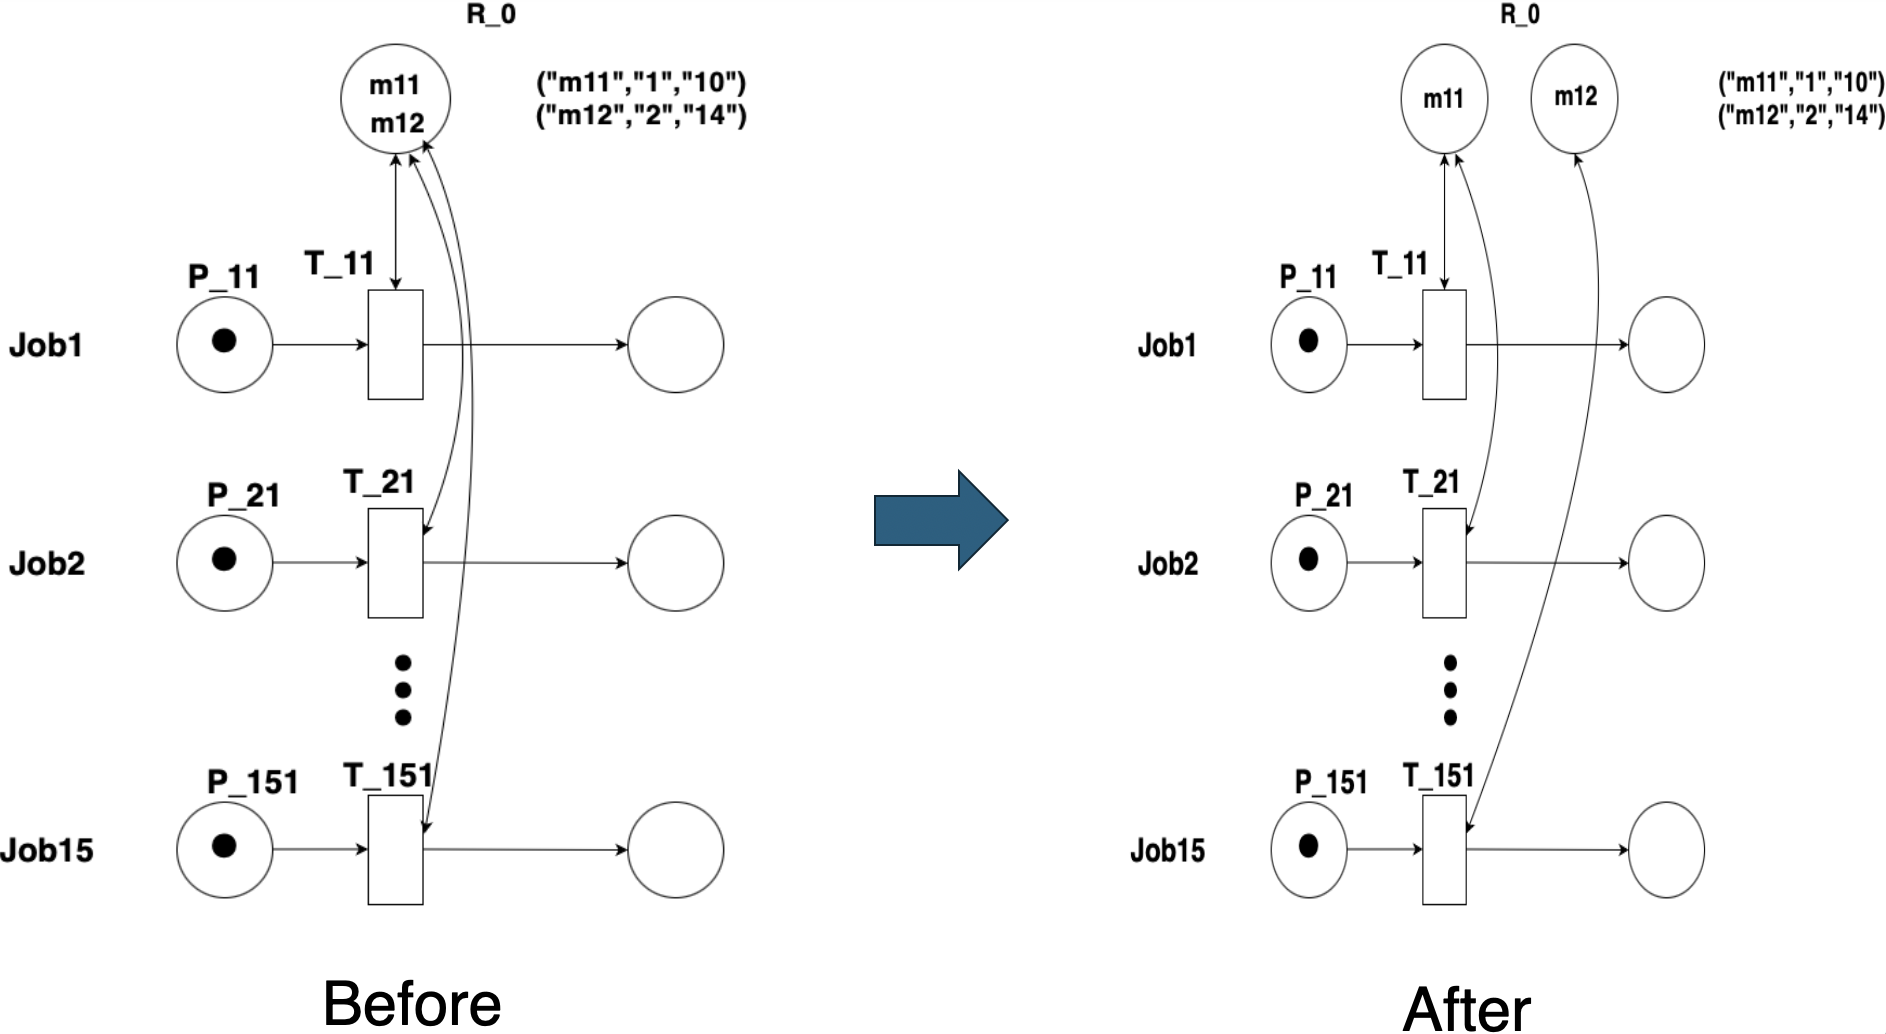
\includegraphics[width=0.8\linewidth, height=7cm]{./images/transformation.png}
    \caption{変数削減のためのペトリネット変換}
    \label{fig:fig5}
\end{figure}

図\ref{fig:fig5}は対象問題のペトリネットモデルを変換した図になる.このモデル変換は以下の二段階のプロセスで構成される.

\begin{enumerate} 
\item リソースの事前割り当てを適用することによりペトリネットモデルを変換する.ペトリネットモデルを変換するためのエネルギー関数が(\ref{eqn:tran})式である.
\begin{align} 
min \sum_{m \ne m_i}^M \left( \sum_t^T a_{m_i,t} \cdot x_{m_i,t} - \sum_t^T a_{m,t} \cdot x_{m,t}\right)^2 + \left(1 - \sum_t^T x_{m,t} \right)^2 \label{eqn:tran} 
\end{align}

\item (\ref{eqn:tran})式をタスクの処理時間またはリソースコストの最適化を行うことで効率的なリソース配置をする.
\end{enumerate}

(\ref{eqn:tran})式の$M$はマシンリソースの集合であり,$T$はタスクの集合である.第一項の目的関数は特定のタスクにおけるあるマシンリソースを基準として他のリソースとの間に差異が生じないようにすることを目的としている.具体的には,タスクの処理時間またはリソースコストの最適化を目的関数とした時に,各リソースの割り当てが均等であることを求めており,リソース間の不均衡を最小化することで全体的なリソースの利用効率を向上させることを目指している.この項は,リソース配分の不均等性による効率的ではない動作を防ぐために最適化において重要な役割を果たす.第二項は制約条件を表しており,1つのタスクに対して2つ以上のマシンリソースが割り当てられないように制限している.この制約は,リソースの重複した割り当てを防ぎ各タスクにおけるリソースの一貫した分配を確保すつことを目的としている.

変数の数は$r \times k \times t$(ここで,$r$はマシンリソース数,$k$は制限の最大時刻,$t$はタスク数)で表される.だが,ペトリネットモデルの変換を行うことにより変数の数が$k \times t$に削減される.この削減により,最適化計算の規模が縮小し計算効率が向上する.

\section{評価実験}
ペトリネットモデルの変換後,3.2と同様な実験を行い比較検証をする.

\subsection{タスク処理時間を最適化したペトリネットモデル変換(戦略1)}

\begin{figure}[H]
    \centering
    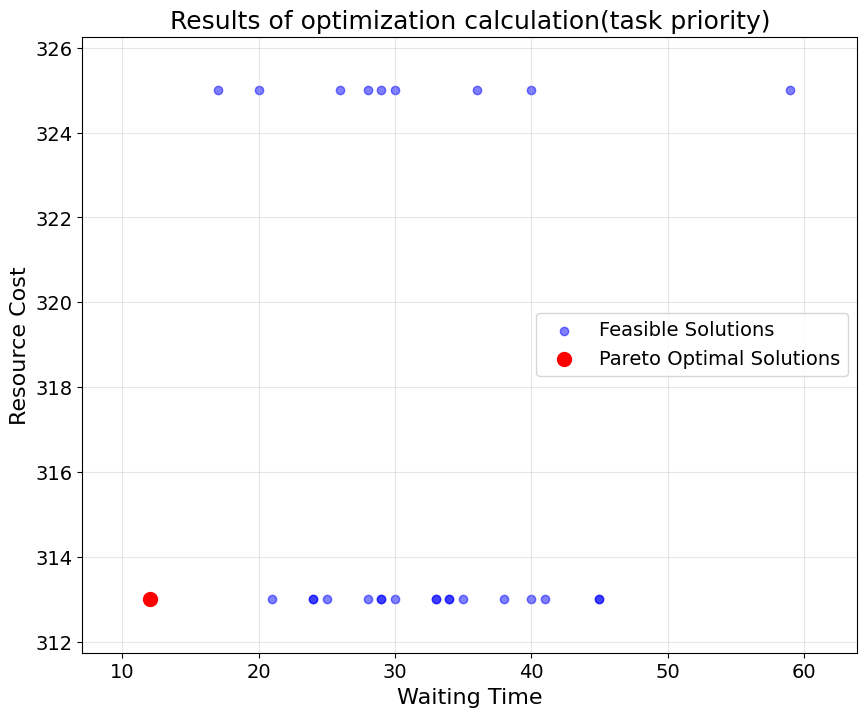
\includegraphics[width=0.8\linewidth, height=8cm]{./images/task_job5.png}
    \caption{タスクの処理時間を最適化したパレート解}
    \label{fig:fig6}
\end{figure}

\begin{table}[ht]
    \centering
    \vspace{-0.3cm}
    \caption{各巡回における実行可能解と個数および平均値(戦略1)}
    \begin{tabular}{|c|c|c|c|}
        \hline
         巡回 & 個数 & Resource Costの平均値 & Waiting Timeの平均値 \\
        \hline
        第1巡 & 7 & 313 & 46.6 \\
        \hline
        第2巡 & 4 & 313 & 32 \\
        \hline
        第3巡 & 6 & 313 & 36.5 \\
        \hline
        第4巡 & 1 & 313 & 20 \\
        \hline
        第5巡 & 4 & 325 & 33.1 \\
        \hline
        全体の平均 & 4.4 & 315.4 & 33.6 \\
        \hline
    \end{tabular}
    \label{tab:task_feasible}
\end{table}

表\ref{tab:task_feasible}は表\ref{tab:before_feasible}と同様に実行可能解の解の分布と解が得られた時のデータを示している.また,図\ref{fig:fig6}はタスク処理時間を最適化した後の最適化計算を行い,得られたパレート解を可視化したグラフになっている.第一段階の最適化において,タスクに使用するマシンリソースの分割を行い,多目的から単目的に変換されるためResource Costが確定される.この段階で分割されたリソースが固定され,第二段階の最適化ではResource Costが一定の値を保ったまま,Waiting Timeの短縮に向けた探索が行われるため解空間上で解が横方向に広がる結果が得られる.ただし,リソースの分割も含めて再計算を行うため全ての解が完全に同一のResource Costを持つわけではなく,一部の解においてResource Costの変動が見られる.

\begin{figure}[H]
    \centering
    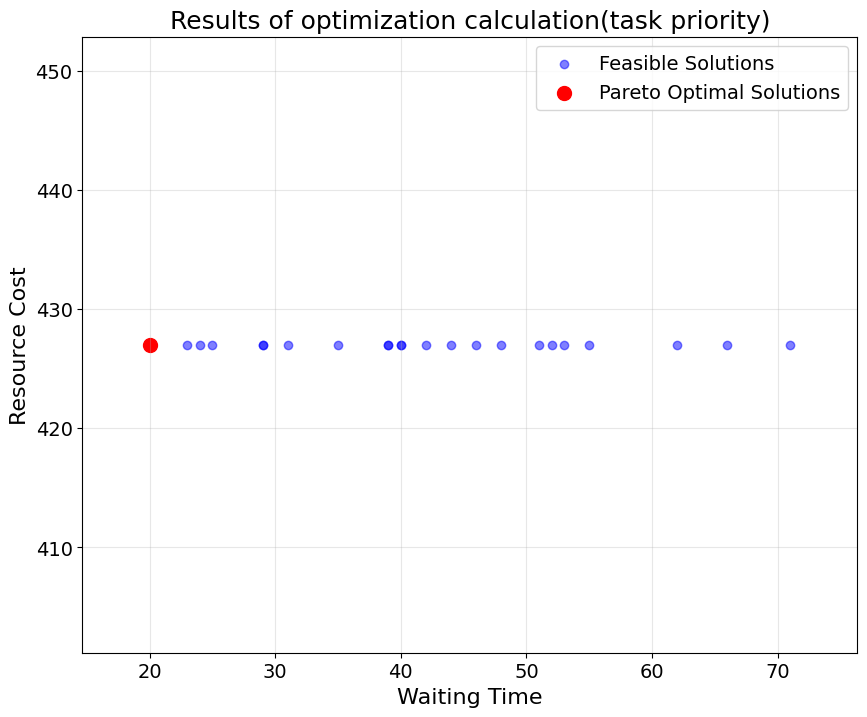
\includegraphics[width=0.8\linewidth, height=8cm]{./images/task_job7.png}
    \caption{戦略1の計算できる最大規模数(job数が7)のパレート解}
    \label{fig:fig7}
\end{figure}
\clearpage

\begin{table}[ht]
    \centering
    \vspace{-0.3cm}
    \caption{戦略1の最大規模数の実行可能解と個数および平均値}
    \begin{tabular}{|c|c|c|c|}
        \hline
         巡回 & 個数 & Resource Costの平均値 & Waiting Timeの平均値 \\
        \hline
        第1巡 & 3 & 427 & 33 \\
        \hline
        第2巡 & 4 & 427 & 39.8 \\
        \hline
        第3巡 & 8 & 427 & 44 \\
        \hline
        第4巡 & 4 & 427 & 50 \\
        \hline
        第5巡 & 4 & 427 & 38.5 \\
        \hline
        全体の平均 & 4.6 & 427 & 41.1 \\
        \hline
    \end{tabular}
    \label{tab:task_feasible_max}
\end{table}

表\ref{tab:task_feasible_max}と図\ref{fig:fig7}は戦略1の計算できる最大規模数(job数が7)の時の結果になっている.job数が5の時と比較して実行可能解が増加している結果は,提案手法が拡大した探索空間を効率的に探索していることを示唆している.モデルの変換前と同様に規模の拡大に伴い目的関数の値の増加が見られる.
 
\subsection{リソースコストを最適化したペトリネットモデル変換(戦略2)}

\begin{figure}[H]
    \centering
    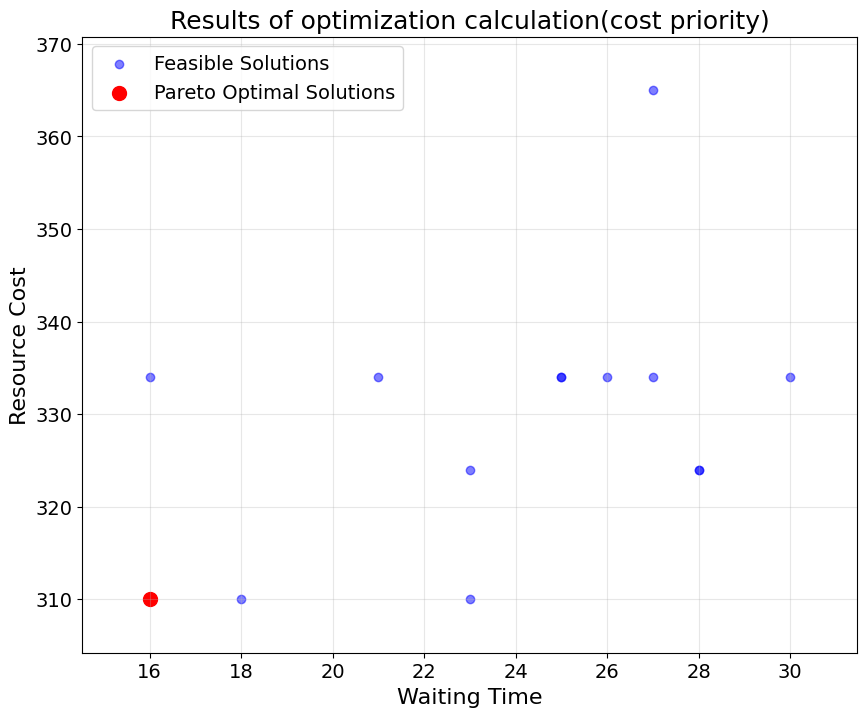
\includegraphics[width=0.8\linewidth, height=8cm]{./images/cost_job5.png}
    \caption{リソースコストを最適化したパレート解}
    \label{fig:fig8}
\end{figure}
\clearpage

\begin{table}[ht]
    \centering
    \vspace{-0.3cm}
    \caption{各巡回における実行可能解と個数および平均値}
    \begin{tabular}{|c|c|c|c|}
        \hline
         巡回 & 個数 & Resource Costの平均値 & Waiting Timeの平均値 \\
        \hline
        第1巡 & 1 & 365 & 27 \\
        \hline
        第2巡 & 3 & 310 & 19 \\
        \hline
        第3巡 & 3 & 324 & 26.3 \\
        \hline
        第4巡 & 0 & - & - \\
        \hline
        第5巡 & 7 & 334 & 24.3 \\
        \hline
        全体の平均 & 3.5 & 333.3 & 24.2 \\
        \hline
    \end{tabular}
    \label{tab:cost_feasible}
\end{table}

表\ref{tab:cost_feasible}は表\ref{tab:task_feasible}と同様に実行可能解の解の分布と解が得られた時のデータを示している.また,図\ref{fig:fig8}はリソースコストの最適化を初段階として行い,解の分布が戦略1で得られた分布と類似していることがわかる.

\begin{figure}[H]
    \centering
    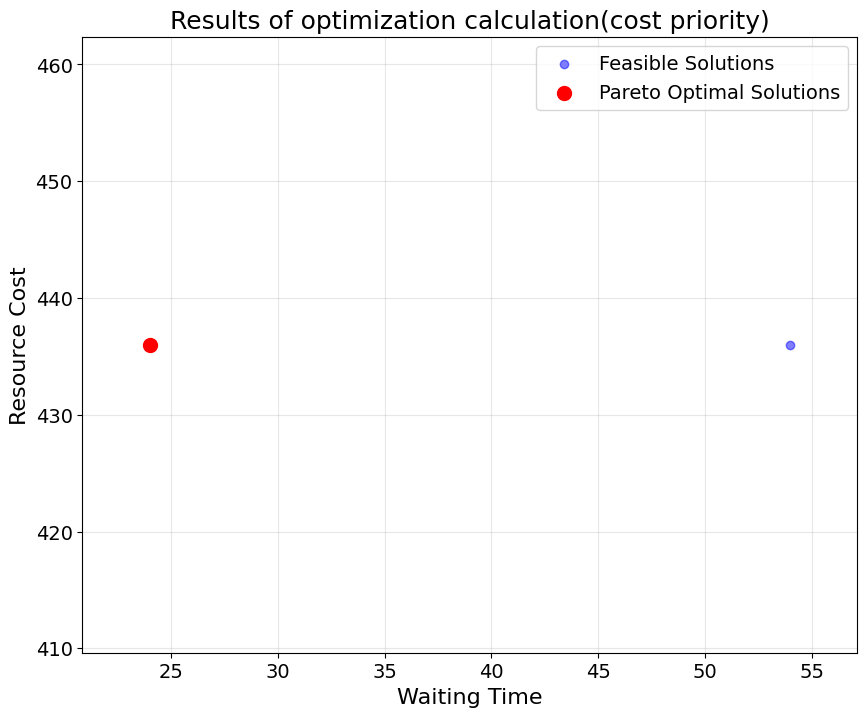
\includegraphics[width=0.8\linewidth, height=8cm]{./images/cost_job7.png}
    \caption{戦略2の計算できる最大規模数(job数が7)のパレート解}
    \label{fig:fig8}
\end{figure}

\begin{table}[ht]
    \centering
    \vspace{-0.3cm}
    \caption{戦略2の最大規模数の実行可能解と個数および平均値}
    \begin{tabular}{|c|c|c|c|}
        \hline
         巡回 & 個数 & Resource Costの平均値 & Waiting Timeの平均値 \\
        \hline
        第1巡 & 0 & - & - \\
        \hline
        第2巡 & 0 & - & - \\
        \hline
        第3巡 & 0 & - & - \\
        \hline
        第4巡 & 0 & - & - \\
        \hline
        第5巡 & 2 & 436 & 39 \\
        \hline
        全体の平均 & 2 & 436 & 39 \\
        \hline
    \end{tabular}
    \label{tab:cost_feasible_max}
\end{table}

表\ref{tab:cost_feasible_max}と図\ref{fig:fig8}は戦略2の計算できる最大規模数(job数が7)の時の結果になっている.job数が5の時と
比較すると実行可能解が減少しているが,戦略1同様規模を拡大しても解を探索することができることより効率的に探索していることを示唆している.

\subsection{ペトリネット変換前と戦略1の比較}
\begin{figure}[H]
    \centering
    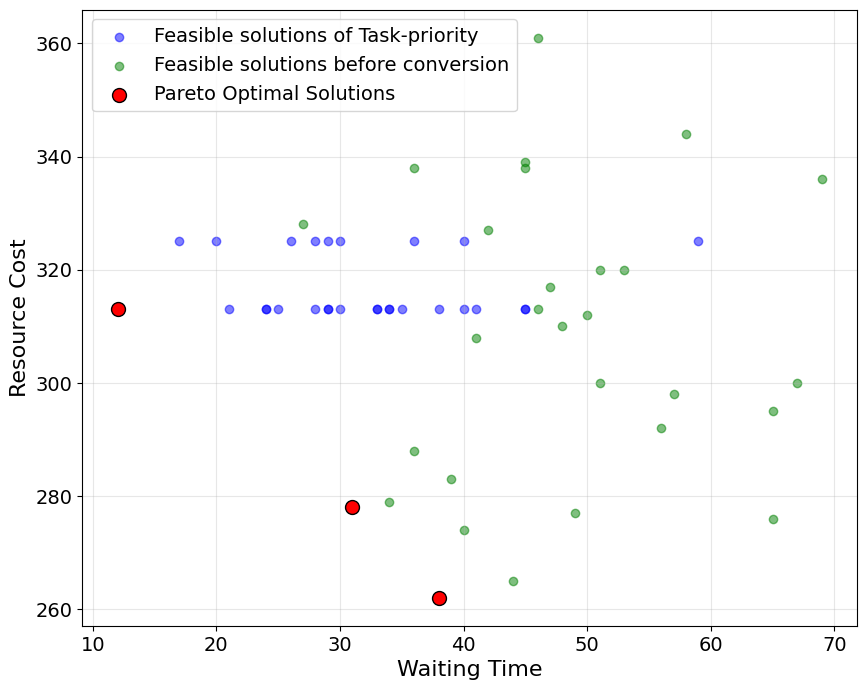
\includegraphics[width=0.8\linewidth, height=8cm]{./images/task_and_before_job5.png}
    \caption{ペトリネット変換前と戦略1のパレート解}
    \label{fig:fig9}
\end{figure}

図\ref{fig:fig9}は,変換を行わない手法と戦略1に基づく最適化計算の結果を同時にプロットしたものである.青の点が戦略1で緑の点が変換前である.この図に示された3つのパレート解のうち,1つは戦略1により得られた解であり,残りの2つは変換を行わない手法による解である.このことから,戦略1においても効率的な解を見つけることが可能であることが示された.また,表\ref{tab:before_feasible}と表\ref{tab:task_feasible}を比較すると,戦略1ではResource Costの値が比較的安定している一方で,変換を行わない手法の結果と比較すると若干劣る傾向が見られる.しかしながら,Waiting Timeに関しては,戦略1の結果において変換を行わない手法の結果と比較して明らかに減少している傾向が確認された.これらの結果は,戦略1がWaiting Timeの最適化に寄与しつつ,Resource Costの安定性を維持できる手法であることを示唆している.

\subsection{ペトリネット変換前と戦略2の比較}
\begin{figure}[H]
    \centering
    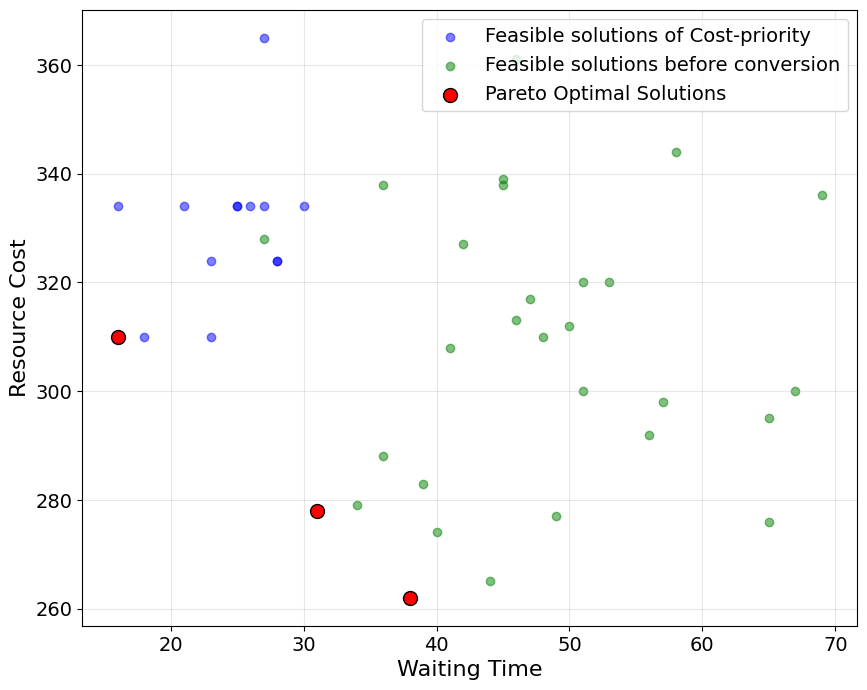
\includegraphics[width=0.8\linewidth, height=8cm]{./images/cost_and_before_job5.png}
    \caption{ペトリネット変換前と戦略2のパレート解}
    \label{fig:fig10}
\end{figure}

図\ref{fig:fig10}は,変換を行わない手法と戦略1に基づく最適化計算の結果を同時にプロットしたものである.戦略1と同様な結果が得られた.このことから,戦略2においても効率的な解を見つけることが可能であることが示された.また,表\ref{tab:before_feasible}と表\ref{tab:cost_feasible}を比較すると,戦略2はWaiting Timeの短縮において顕著な効果を示していることが明らかとなった.一方で,Resource Costが増加し,実行可能解の個数が減少している点は,課題として考慮する必要がある.

\section{考察}
変換手法の戦略1および戦略2において観察された実行可能解の減少は,モデル変換によって導入された付加的な制約条件に起因するものと考えられる.この実行可能解の減少が一見すると解の多様性の損失として捉えられる可能性があるが,むしろ質的な観点からは有意義な減少である可能性があると示唆される.具体的には,戦略1および戦略2の適用により,システムにおけるWaiting Timeが統計的に有意な減少を示したことが確認されている.このことから,スケジューリング戦略が制約条件を厳格化することで低品質な解を排除し,より効率的で質の高い解を優先するように探索空間を調整したことを示唆している.一方で,実行可能解の減少に伴う探索空間の縮小がResource Costの増加と関連している可能性も考えられる.制約条件の厳格化により,低コストな解が探索区間から排除された結果Resource Costが増加したと推測される.

さらに,本研究ではモデル変換を適用することで問題の規模が大きくなった場合でも計算を実行可能であることが示された.この結果は,変数数の削減や探索効率の向上を通じてモデル変換がスケーラビリティの向上に寄与していることを示唆していると思われる.また,モデル変換後においてリソースコストを優先した場合よりもタスクの処理時間を優先した場合の方が実行可能解の個数が多かった理由として,マシンリソースの性能とコストのばらつきが影響していると考えられる.具体的には,タスクの処理時間を優先する場合,性能の高いマシンが優先的に活用されることでスケジュールが柔軟に調整され多くの実行可能解が得られたと推測される.一方で,リソースコストを優先する場合,探索空間に厳格な制約が課されその結果,より効率的なスケジューリングが可能な良質な解が排除されてしまい実行可能解の個数が減少したと考えられる。

また,本研究で提案された戦略1および戦略2は,特にWaiting Timeの最小化が重要視される運用システムにおいて有力なスケジューリング戦略となり得る.このことは,システムの要求事項や運用目的に応じた柔軟で適応的なアプローチの重要性を強調している.一方で,Resource Costの増加が一定の課題として残るため,より広い解空間を確保する探索手法の導入や,制約条件の緩和を検討する余地がある.
